\chapter{Results}

In this chapter, attained results during the development of this project will be
presented. First, a series of benchmarks have been used in order to exercise key
Alcaudon modules and measure how the system behaves. Then, a possible real
application for Alcaudon will be stated. To conclude, a summary of accomplished
objectives is presented.

\section{Benchmarks}

Alcaudon has been tested thoroughly, both using traditional testing techniques
as well as more state-of-the-art techniques such as property based testing.
These tests can guarantee correctness in terms of behavior, but they do not
measure system precision in terms of performance goals. Even though Alcaudon
has been designed carefully, using the adequate data structures and taking
care of performance, empiric results are needed. It is known that creating
accurate benchmarks is complex~\cite{benchbias}, as there are many factors
that can lead to misleading results. Presented benchmarks are implemented using
JMH\footnote{http://openjdk.java.net/projects/code-tools/jmh/}.

\subsection{Computation execution benchmark}

This benchmark measures the number of computations per second that Alcaundon can
handle.

\begin{lstlisting}
# JMH version: 1.19
# VM version: JDK 1.8.0_131, VM 25.131-b11
# VM invoker: /usr/lib/jvm/java-8-oracle/jre/bin/java
# VM options: <none>
# Warmup: 15 iterations, 1 s each
# Measurement: 15 iterations, 1 s each
# Timeout: 10 min per iteration
# Threads: 1 thread, will synchronize iterations
# Benchmark mode: Throughput, ops/time
# Benchmark: org.alcaudon.runtime.ComputationBenchmark.throughput

# Fork: 1 of 1
# Warmup Iteration   1: 2838.544 ops/s
# Warmup Iteration   2: 12645.095 ops/s
# Warmup Iteration   3: 13336.237 ops/s
# Warmup Iteration   4: 15380.058 ops/s
# Warmup Iteration   5: 16003.125 ops/s
# Warmup Iteration   6: 15388.756 ops/s
# Warmup Iteration   7: 14816.361 ops/s
# Warmup Iteration   8: 14820.269 ops/s
# Warmup Iteration   9: 14826.327 ops/s
# Warmup Iteration  10: 15995.409 ops/s
# Warmup Iteration  11: 17395.065 ops/s
# Warmup Iteration  12: 17396.909 ops/s
# Warmup Iteration  13: 16674.274 ops/s
# Warmup Iteration  14: 16668.055 ops/s
# Warmup Iteration  15: 16668.801 ops/s
Iteration   1: 16006.082 ops/s
Iteration   2: 16021.392 ops/s
Iteration   3: 16002.350 ops/s
Iteration   4: 16673.828 ops/s
Iteration   5: 16002.128 ops/s
Iteration   6: 13795.418 ops/s
Iteration   7: 14293.416 ops/s
Iteration   8: 12902.619 ops/s
Iteration   9: 14826.131 ops/s
Iteration  10: 14279.800 ops/s
Iteration  11: 14834.078 ops/s
Iteration  12: 13347.936 ops/s
Iteration  13: 14818.898 ops/s
Iteration  14: 14811.602 ops/s
Iteration  15: 14286.494 ops/s


Result "org.alcaudon.runtime.ComputationBenchmark.throughput":
  14860.145 ±(99.9%) 1171.277 ops/s [Average]
  (min, avg, max) = (12902.619, 14860.145, 16673.828), stdev = 1095.613
  CI (99.9%): [13688.868, 16031.422] (assumes normal distribution)
\end{lstlisting}

\subsection{Stream benchmark}

This benchmark measures the number of records that a stream can handle using
the network stack.

\begin{lstlisting}
# JMH version: 1.19
# VM version: JDK 1.8.0_131, VM 25.131-b11
# VM invoker: /usr/lib/jvm/java-8-oracle/jre/bin/java
# VM options: <none>
# Warmup: 15 iterations, 1 s each
# Measurement: 15 iterations, 1 s each
# Timeout: 10 min per iteration
# Threads: 1 thread, will synchronize iterations
# Benchmark mode: Throughput, ops/time
# Benchmark: org.alcaudon.runtime.StreamBenchmark.throughput

# Fork: 1 of 1
# Warmup Iteration   1: 9321.185 ops/s
# Warmup Iteration   2: 31098.503 ops/s
# Warmup Iteration   3: 56383.813 ops/s
# Warmup Iteration   4: 89775.005 ops/s
# Warmup Iteration   5: 92496.201 ops/s
# Warmup Iteration   6: 66532.817 ops/s
# Warmup Iteration   7: 56076.426 ops/s
# Warmup Iteration   8: 63003.972 ops/s
# Warmup Iteration   9: 59410.283 ops/s
# Warmup Iteration  10: 58177.190 ops/s
# Warmup Iteration  11: 59273.481 ops/s
# Warmup Iteration  12: 61445.394 ops/s
# Warmup Iteration  13: 52879.995 ops/s
# Warmup Iteration  14: 57380.524 ops/s
# Warmup Iteration  15: 46046.720 ops/s
Iteration   1: 69487.193 ops/s
Iteration   2: 28153.126 ops/s
Iteration   3: 65117.851 ops/s
Iteration   4: 51256.389 ops/s
Iteration   5: 44682.554 ops/s
Iteration   6: 43606.471 ops/s
Iteration   7: 31458.501 ops/s
Iteration   8: 66222.260 ops/s
Iteration   9: 61828.791 ops/s
Iteration  10: 24873.576 ops/s
Iteration  11: 58282.826 ops/s
Iteration  12: 61180.519 ops/s
Iteration  13: 12427.225 ops/s
Iteration  14: 55291.714 ops/s
Iteration  15: 38296.842 ops/s

Result "org.alcaudon.runtime.StreamBenchmark.throughput":
  47477.722 +-(99.9%) 18537.348 ops/s [Average]
  (min, avg, max) = (12427.225, 47477.722, 69487.193), stdev = 17339.847
  CI (99.9%): [28940.375, 66015.070] (assumes normal distribution)
\end{lstlisting}

\subsection{Record router benchmark}

This benchmark measures the number of records that a router can route.

\begin{lstlisting}
# JMH version: 1.19
# VM version: JDK 1.8.0_131, VM 25.131-b11
# VM invoker: /usr/lib/jvm/java-8-oracle/jre/bin/java
# VM options: <none>
# Warmup: 15 iterations, single-shot each
# Measurement: 15 iterations, single-shot each
# Timeout: 10 min per iteration
# Threads: 1 thread
# Benchmark mode: Single shot invocation time
# Benchmark: org.alcaudon.KeyRouterBenchmark.timePerRoute

# Fork: 1 of 1
# Warmup Iteration   1: 381472.618 us/op
# Warmup Iteration   2: 150042.661 us/op
# Warmup Iteration   3: 176778.359 us/op
# Warmup Iteration   4: 106955.031 us/op
# Warmup Iteration   5: 99704.939 us/op
# Warmup Iteration   6: 57248.973 us/op
# Warmup Iteration   7: 37281.762 us/op
# Warmup Iteration   8: 85989.580 us/op
# Warmup Iteration   9: 23317.259 us/op
# Warmup Iteration  10: 33628.435 us/op
# Warmup Iteration  11: 23899.475 us/op
# Warmup Iteration  12: 22373.551 us/op
# Warmup Iteration  13: 22630.460 us/op
# Warmup Iteration  14: 22016.820 us/op
# Warmup Iteration  15: 21163.906 us/op
Iteration   1: 23386.227 us/op
Iteration   2: 26890.087 us/op
Iteration   3: 27592.136 us/op
Iteration   4: 25660.356 us/op
Iteration   5: 26705.218 us/op
Iteration   6: 49419.625 us/op
Iteration   7: 54298.073 us/op
Iteration   8: 116075.003 us/op
Iteration   9: 28676.928 us/op
Iteration  10: 19761.540 us/op
Iteration  11: 19466.265 us/op
Iteration  12: 23165.587 us/op
Iteration  13: 18574.349 us/op
Iteration  14: 21910.841 us/op
Iteration  15: 20325.704 us/op


Result "org.alcaudon.KeyRouterBenchmark.timePerRoute":
  N = 15
  mean =  33460.529 +-(99.9%) 26862.874 us/op

  Histogram, us/op:
    [ 10000.000,  20000.000) = 3
    [ 20000.000,  30000.000) = 9
    [ 30000.000,  40000.000) = 0
    [ 40000.000,  50000.000) = 1
    [ 50000.000,  60000.000) = 1
    [ 60000.000,  70000.000) = 0
    [ 70000.000,  80000.000) = 0
    [ 80000.000,  90000.000) = 0
    [ 90000.000, 100000.000) = 0
    [100000.000, 110000.000) = 0

  Percentiles, us/op:
      p(0.0000) =  18574.349 us/op
     p(50.0000) =  25660.356 us/op
     p(90.0000) =  79008.845 us/op
     p(95.0000) = 116075.003 us/op
     p(99.0000) = 116075.003 us/op
     p(99.9000) = 116075.003 us/op
     p(99.9900) = 116075.003 us/op
     p(99.9990) = 116075.003 us/op
     p(99.9999) = 116075.003 us/op
    p(100.0000) = 116075.003 us/op
\end{lstlisting}

\section{Alcaudon application}

Once Alcaudon has been described in detail, its full potential can be unveiled
in a real world scenario. For this example, a
public\footnote{http://www.nyc.gov/html/tlc} data set of the New York City Taxi
and Limousine Commission (TLC) will be used. This data set contains records
about taxi trips in New York from different years. The goal of this example is
to use this data set as a real unbounded data source, where taxi customers take
taxis for a ride from point A to point B and this information is delivered into
Alcaudon. With this information it is possible to build an Alcaudon dataflow
topology in order to detect spikes in rides to certain parts of the city, for
example during a concert. For companies like Uber, where prices fluctuate
depending on demand, processing this information in \textit{real time} is
fundamental. This example will build an Alcaudon dataflow topology in order to
aggregate rides per zone and emit results in constant time windows. These
aggregated results will be published into ElasticSearch to be visualized later
on as shown in figure~\ref{fig:rides}. Business stakeholders can use these
dashboards in order to take decisions with the latest information available.

\begin{figure}[!h]
\begin{center}
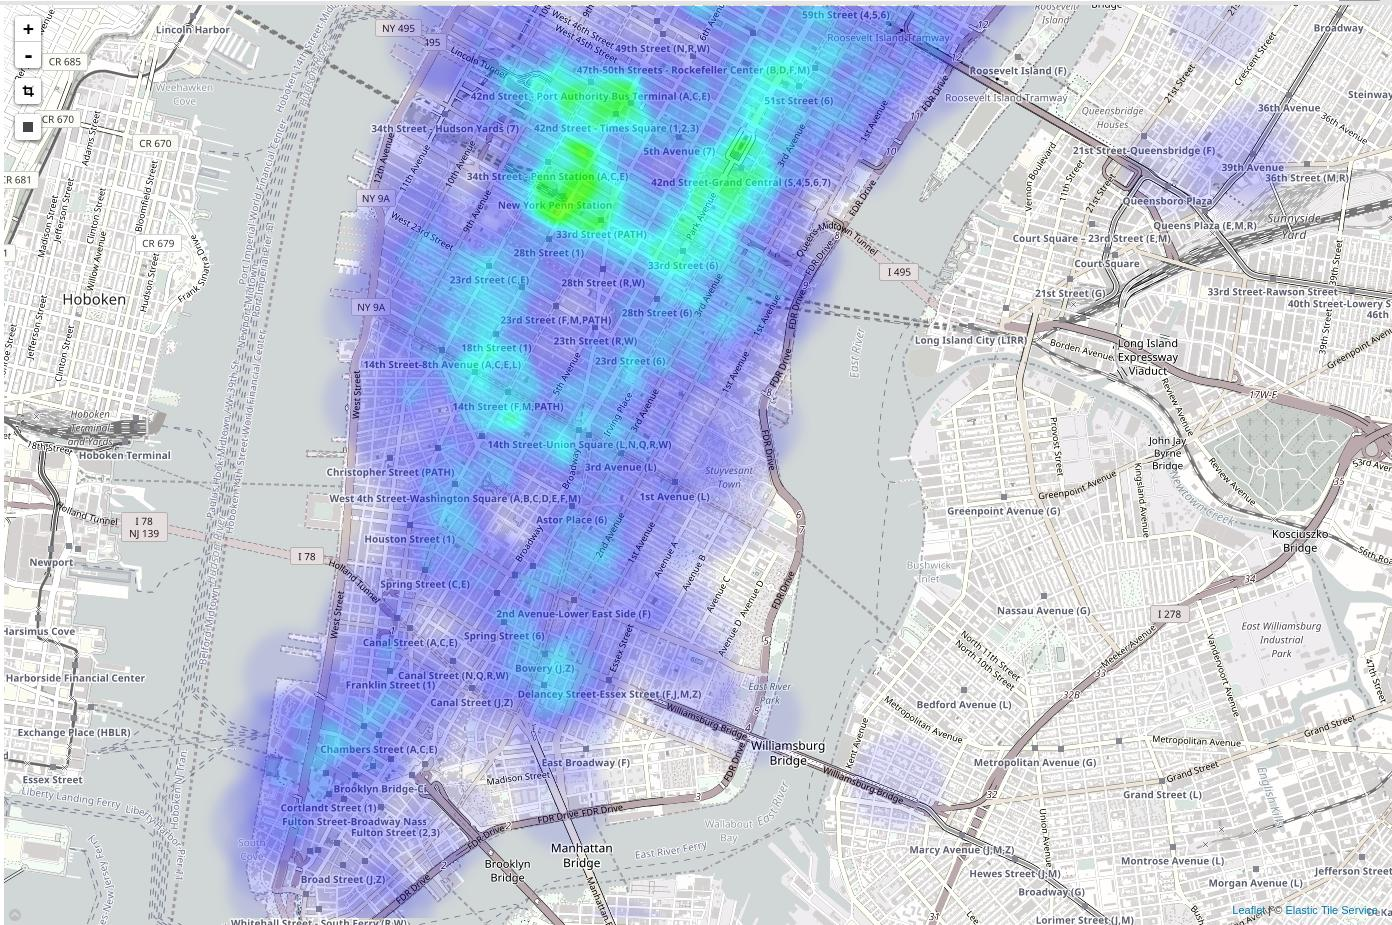
\includegraphics[width=0.8\textwidth]{nyrides.jpg}
\caption{Example dashboard}
\label{fig:rides}
\end{center}
\end{figure}

Since this is a synthetic example, a custom source has been defined in order to
emit ride events using their original timestamps. Ride information contains
different fields, but for the purposes of this example, a simple representation
has been created, listed in~\ref{code:ride}. In order to aggregate location
information, the map is divided into cells, where each ride belongs to one of
these cells. This subdivision in cells is used in order to define a key per
record as it can be found in listing~\ref{code:keyExtractorNY}.

The main goal of this example is to publish updated data about the number of
passengers taking rides in different places of the city, to later on visualize
this data in a dashboard. First of all, rides that are not taking place in New
York are filtered out~(\ref{code:computationFilterRide}) and published into a new
stream. These filtered rides are consumed by
RidePassengerCountComputation~\ref{code:computationRide} that is responsible
for keeping track of the number of passengers per cell and updating them when new rides
arrive into the system. A timer is set-up, when this timer is triggered, the
information stored up to that point, in this case the number of ride passengers
per cell, is published into a Sink. In addition to counting the number of
passengers, this computation publishes into a different sink when the number of
passengers arriving into a specific cell is bigger than a setting. This is
useful when alerts for different events are needed. Dataflow topology definition
can be found in listing~\ref{code:rideDataflow}. This example shows the
potential of unbounded data-set processing, and the strengths of Alcaudon in
particular.

\begin{lstlisting}[language=scala, frame=trBL, label=code:ride, float=ht, caption = {Ride \acs{ADT}}]
case class Ride(id: Long, time: DateTime, location: Point, passengerCount: Int)
\end{lstlisting}

\begin{lstlisting}[language=scala, frame=trBL, label=code:computationFilterRide, float=ht, caption = {Computation to filter out non New York rides}]
class FilterRideComputation extends Computation {
  def processRecord(record: Record): Unit = {
    val ride: Ride = deserialize(record.value)
    if (ride.isInNYC())
      produceRecord(nycRides, record)
  }

  def processTimer(timeStamp: Timer): Unit = {}
}
\end{lstlisting}

\begin{lstlisting}[language=scala, frame=trBL, label=code:keyExtractorNY, float=ht, caption = {Key extractor function}]
class RideKeyExtractor extends KeyExtractor {
  def extractKey(msg: Array[Byte]): String = {
    val ride: Ride = deserialize(msg)
    Utils.locationToCell(ride.location)
  }
}
\end{lstlisting}

\begin{lstlisting}[language=scala, frame=trBL, label=code:computationRide, float=ht, caption = {Ride \acs{ADT}}]
class RidePassengerCountComputation extends Computation {
  def processRecord(record: Record): Unit = {
    val ride: Ride = deserialize(record.value)
    val count: Int = get(record.key) + ride.passengerCount
    if (count > settings.alertPassengers)
      produceRecord(alertSink, RawRecord(serialize(record.key), record.timestamp))
    set(count + ride.passengerCount)
    setTimer(FixedRecurrentTimer(cell, 5.minutes))
  }

  def processTimer(timeStamp: Timer): Unit = {
    val location = Utils.cellToLocation(timer.tag)
    val totalPassengerCount = get(timer.tag)
    produceRecord(elasticSink, RawRecord(serialize((location, totalPassengerCount)), record.timestamp))
  }
}
\end{lstlisting}

\begin{lstlisting}[language=scala, frame=trBL, label=code:rideDataflow, float=ht, caption = {Ride dataflow creation}]
val dataflow = DataflowBuilder("ridesCounter")
  .withSource("taxiRides", TaxiRides())
  .withComputation("filterNYRides",
    FilterRideComputation,
    OutputStreams("nycRides"),
    AlcaudonInputStream("taxiRides")
  .withComputation("passengerCount",
    RidePassengerCountComputation,
    OutputStreams("elasticSink", "alertSink"),
    AlcaudonInputStream("nycRides", new RideKeyExtractor())
  .withSink("elasticSink", ElasticSearchSink)
  .withSink("alertSink", HTTPSink(settings.alertEndpoint))
  .build()
\end{lstlisting}

\section{Accomplished objectives}

During the development of this project, all objectives defined at the beginning
of this document have been accomplished. Alcaudon provides all the necessary
tools to deploy distributed stream data processing pipelines. It attains this
objective by supplying an abstract model, the Computation \acs{API}, that users
implement, leveraging the all the complexities around fault-tolerant distributed
models to Alcaudon.

Regarding specific objectives, these have been accomplished as well:
%
\begin{itemize}
\item Alcaudon provides an abstraction in order to create distributed
  computations; computation \acs{API} alongside the dataflow builder.
\item The system provides exactly-once processing semantics, using at-least once
  delivery in combination with idempotent record processing. In order to achieve
  idempotence, state-of-the-art probabilistic data structures have been used as
  well as persistent actors to guarantee persistent state durability.
\item The system provides watermark based timers in order to work with
  out-of-order data. The implementation of this subsystem uses state-of-the-art
  coordination-free distributed data types in order to replicate knowledge about
  time event evolution inside the system.
\item Dataflow \acs{DAG}s are scheduled into available compute nodes using an
  state-of-the-art flexible cluster scheduler~\cite{firmament}. Different scheduling
  policies can be configured depending on the needs, where the default choice is
  biased towards co-location.
\item Several sources and sinks are provided by default such as Twitter streaming
  API, TCP Sockets or Apache Kafka. However it is possible to implement new ones
  just extending SourceFn and SinkFN interfaces.
\item Alcaudon provides an elastic distributed implementation where compute
  nodes can join the cluster in the events of burst of load. The system has been
  designed in order to be resilient and fault-tolerant. The actor model has
  facilitated the development in terms of resilience due to is supervision mechanism that
  allows to isolate failure.
\item Alcaudon provides different metrics about the state of the system. It has been
  integrated with industry proven technologies in the space of monitoring such as
  Prometheus and Graphana. Using these tools it is possible to create a rich set
  of alerts and dashboards giving a good overview of how the different components
  of Alcaudon perform.
\item Alongside the previously presented results, Alcaudon is distributed using Docker
  containers and its library is available in SonaType repository. This makes almost
  trivial to deploy a full-featured Alcaudon cluster.
\end{itemize}

\section{Future work}

Given that Alcaudon has been designed in a modular way and it has many automatic
tests, including new features should be effortless. In this section some future work
that could be done to the platform is presented.

\begin{itemize}
\item Improve system performance avoiding object allocations in certain
  sensitive parts of the system such as the Streams. High allocation rate
  usually hurts managed systems performance due to garbage collection. Some
  systems such as Netty\footnote{https://netty.io/} use pre-allocated memory buffers
  in order to avoid heap allocations as much as possible. This approach could be
  explored in order to improve Alcaudon performance.
\item Implement a machine learning algorithm in order to select a scheduling policy
  based on similar already run dataflow pipelines, improving the overall performance.
\item Implement a fully functional programming interface on top of the
  computation API in order to offer a more expressive API to the users.
  Providing \textit{combinators} such as map, groupBy, filter, etc.
\item Alcaudon watermark algorithm is just a minimal version. Used heuristic
  could be improved and it would be interesting to test different machine
  learning algorithms in order to predict watermarks. Another interesting
  approach to the problem that watermarks solve is to use virtual tables as
  Apache Kafka Streaming does~\cite{kafkastreams}.
\end{itemize}
